\documentclass{standalone}
\usepackage{tikz}
\usetikzlibrary{patterns, positioning}

\begin{document}
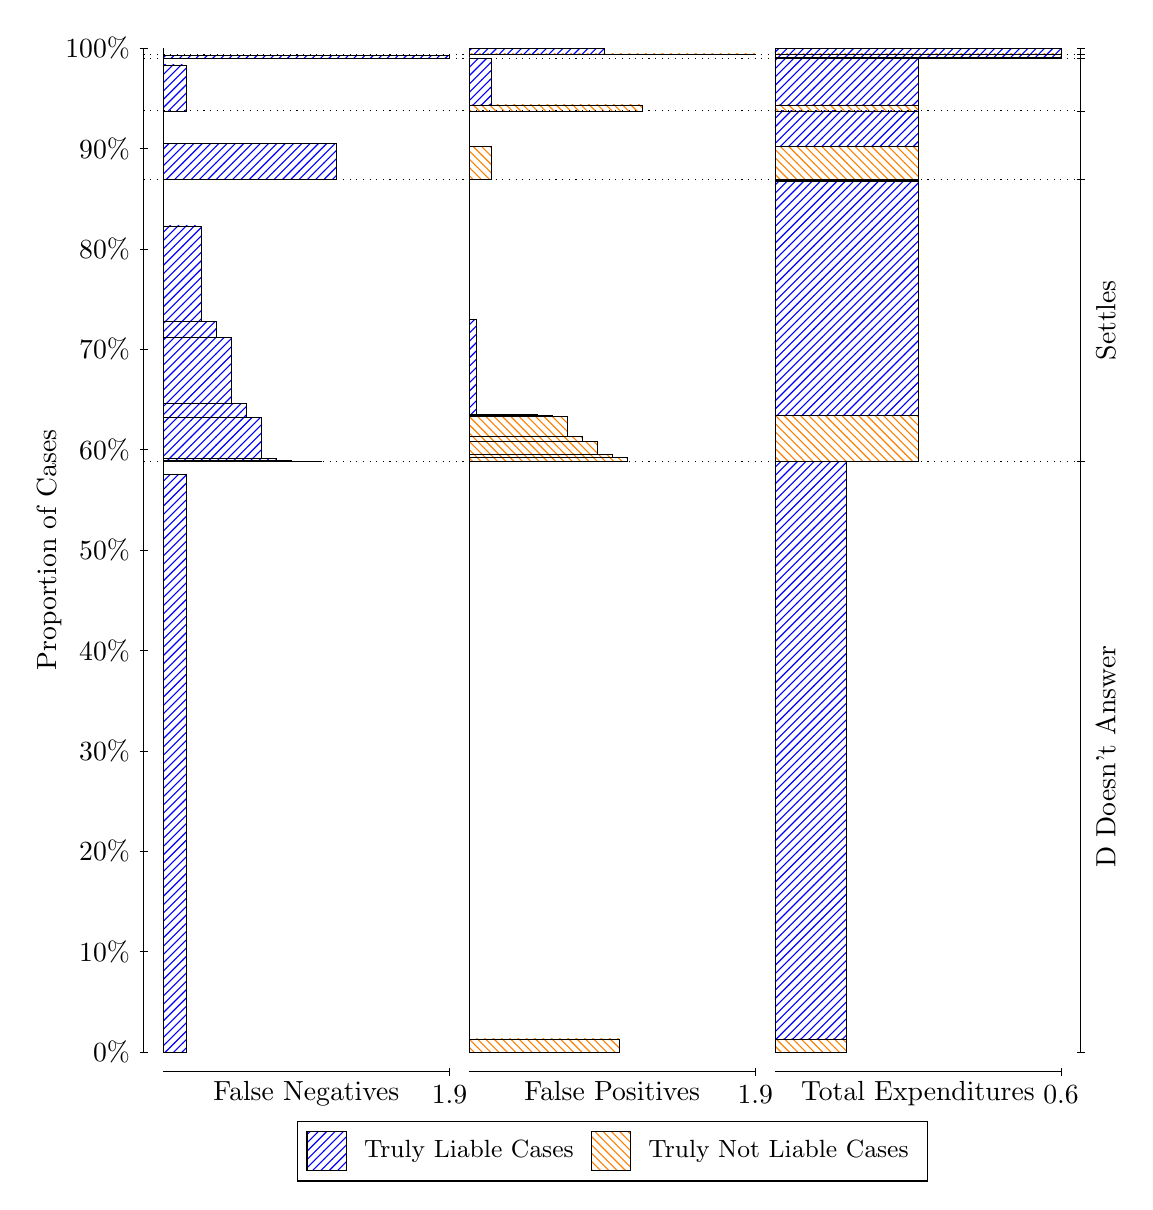
\begin{tikzpicture}
\draw[black, very thin] (1.5,1.75) -- (1.5,14.5);
\node[rotate=90, anchor=center] at (0.3, 8.125) {Proportion of Cases};
\draw[black, very thin] (1.45,1.75) -- (1.55,1.75);
\node[anchor=east] at (1.45, 1.75) {0\%};
\draw[black, very thin] (1.45,3.025) -- (1.55,3.025);
\node[anchor=east] at (1.45, 3.025) {10\%};
\draw[black, very thin] (1.45,4.3) -- (1.55,4.3);
\node[anchor=east] at (1.45, 4.3) {20\%};
\draw[black, very thin] (1.45,5.575) -- (1.55,5.575);
\node[anchor=east] at (1.45, 5.575) {30\%};
\draw[black, very thin] (1.45,6.85) -- (1.55,6.85);
\node[anchor=east] at (1.45, 6.85) {40\%};
\draw[black, very thin] (1.45,8.125) -- (1.55,8.125);
\node[anchor=east] at (1.45, 8.125) {50\%};
\draw[black, very thin] (1.45,9.4) -- (1.55,9.4);
\node[anchor=east] at (1.45, 9.4) {60\%};
\draw[black, very thin] (1.45,10.675) -- (1.55,10.675);
\node[anchor=east] at (1.45, 10.675) {70\%};
\draw[black, very thin] (1.45,11.95) -- (1.55,11.95);
\node[anchor=east] at (1.45, 11.95) {80\%};
\draw[black, very thin] (1.45,13.225) -- (1.55,13.225);
\node[anchor=east] at (1.45, 13.225) {90\%};
\draw[black, very thin] (1.45,14.5) -- (1.55,14.5);
\node[anchor=east] at (1.45, 14.5) {100\%};

\draw[black, very thin] (13.4,1.75) -- (13.4,14.5);
\draw[black, very thin] (13.35,1.75) -- (13.45,1.75);
\node[anchor=west] at (13.35, 1.75) {};
\draw[black, very thin] (13.35,9.2517) -- (13.45,9.2517);
\node[anchor=west] at (13.35, 9.2517) {};
\draw[black, very thin] (13.35,12.836) -- (13.45,12.836);
\node[anchor=west] at (13.35, 12.836) {};
\draw[black, very thin] (13.35,13.702) -- (13.45,13.702);
\node[anchor=west] at (13.35, 13.702) {};
\draw[black, very thin] (13.35,14.364) -- (13.45,14.364);
\node[anchor=west] at (13.35, 14.364) {};
\draw[black, very thin] (13.35,14.421) -- (13.45,14.421);
\node[anchor=west] at (13.35, 14.421) {};
\draw[black, very thin] (13.35,14.5) -- (13.45,14.5);
\node[anchor=west] at (13.35, 14.5) {};

\draw[black, very thin, pattern color=blue, pattern=north east lines] (1.75,1.75) rectangle (2.0368,9.0847);
\draw[black, very thin, pattern color=orange, pattern=north west lines] (1.75,9.0847) rectangle (1.75,9.2517);
\draw[black, very thin, pattern color=blue, pattern=north east lines] (1.75,9.2517) rectangle (3.7579,9.2537);
\draw[black, very thin, pattern color=blue, pattern=north east lines] (1.75,9.2537) rectangle (3.5667,9.2546);
\draw[black, very thin, pattern color=blue, pattern=north east lines] (1.75,9.2546) rectangle (3.3754,9.2645);
\draw[black, very thin, pattern color=blue, pattern=north east lines] (1.75,9.2645) rectangle (3.1842,9.2853);
\draw[black, very thin, pattern color=blue, pattern=north east lines] (1.75,9.2853) rectangle (2.993,9.81);
\draw[black, very thin, pattern color=blue, pattern=north east lines] (1.75,9.81) rectangle (2.8018,9.9886);
\draw[black, very thin, pattern color=blue, pattern=north east lines] (1.75,9.9886) rectangle (2.6105,10.824);
\draw[black, very thin, pattern color=blue, pattern=north east lines] (1.75,10.824) rectangle (2.4193,11.03);
\draw[black, very thin, pattern color=blue, pattern=north east lines] (1.75,11.03) rectangle (2.2281,12.241);
\draw[black, very thin, pattern color=orange, pattern=north west lines] (1.75,12.241) rectangle (1.75,12.836);
\draw[black, very thin, pattern color=blue, pattern=north east lines] (1.75,12.836) rectangle (3.9491,13.287);
\draw[black, very thin, pattern color=orange, pattern=north west lines] (1.75,13.287) rectangle (1.75,13.702);
\draw[black, very thin, pattern color=blue, pattern=north east lines] (1.75,13.702) rectangle (2.0368,14.286);
\draw[black, very thin, pattern color=orange, pattern=north west lines] (1.75,14.286) rectangle (1.75,14.364);
\draw[black, very thin, pattern color=blue, pattern=north east lines] (1.75,14.364) rectangle (5.3833,14.404);
\draw[black, very thin, pattern color=orange, pattern=north west lines] (1.75,14.404) rectangle (1.75,14.421);
\draw[black, very thin, pattern color=orange, pattern=north west lines] (1.75,14.421) rectangle (1.75,14.425);
\draw[black, very thin, pattern color=blue, pattern=north east lines] (1.75,14.425) rectangle (1.75,14.5);
\draw[black, very thin, pattern color=orange, pattern=north west lines] (5.6333,1.75) rectangle (7.5456,1.917);
\draw[black, very thin, pattern color=blue, pattern=north east lines] (5.6333,1.917) rectangle (5.6333,9.2517);
\draw[black, very thin, pattern color=orange, pattern=north west lines] (5.6333,9.2517) rectangle (7.6412,9.2979);
\draw[black, very thin, pattern color=orange, pattern=north west lines] (5.6333,9.2979) rectangle (7.45,9.3361);
\draw[black, very thin, pattern color=orange, pattern=north west lines] (5.6333,9.3361) rectangle (7.2588,9.5022);
\draw[black, very thin, pattern color=orange, pattern=north west lines] (5.6333,9.5022) rectangle (7.0675,9.5721);
\draw[black, very thin, pattern color=orange, pattern=north west lines] (5.6333,9.5721) rectangle (6.8763,9.8216);
\draw[black, very thin, pattern color=orange, pattern=north west lines] (5.6333,9.8216) rectangle (6.6851,9.8367);
\draw[black, very thin, pattern color=orange, pattern=north west lines] (5.6333,9.8367) rectangle (6.6851,9.8372);
\draw[black, very thin, pattern color=orange, pattern=north west lines] (5.6333,9.8372) rectangle (6.4939,9.8449);
\draw[black, very thin, pattern color=orange, pattern=north west lines] (5.6333,9.8449) rectangle (6.3026,9.8454);
\draw[black, very thin, pattern color=orange, pattern=north west lines] (5.6333,9.8454) rectangle (6.1114,9.8469);
\draw[black, very thin, pattern color=blue, pattern=north east lines] (5.6333,9.8469) rectangle (5.7289,11.058);
\draw[black, very thin, pattern color=blue, pattern=north east lines] (5.6333,11.058) rectangle (5.6333,12.836);
\draw[black, very thin, pattern color=orange, pattern=north west lines] (5.6333,12.836) rectangle (5.9202,13.25);
\draw[black, very thin, pattern color=blue, pattern=north east lines] (5.6333,13.25) rectangle (5.6333,13.702);
\draw[black, very thin, pattern color=orange, pattern=north west lines] (5.6333,13.702) rectangle (7.8325,13.779);
\draw[black, very thin, pattern color=blue, pattern=north east lines] (5.6333,13.779) rectangle (5.9202,14.364);
\draw[black, very thin, pattern color=orange, pattern=north west lines] (5.6333,14.364) rectangle (5.6333,14.38);
\draw[black, very thin, pattern color=blue, pattern=north east lines] (5.6333,14.38) rectangle (5.6333,14.421);
\draw[black, very thin, pattern color=orange, pattern=north west lines] (5.6333,14.421) rectangle (9.2667,14.425);
\draw[black, very thin, pattern color=blue, pattern=north east lines] (5.6333,14.425) rectangle (7.3544,14.5);
\draw[black, very thin, pattern color=orange, pattern=north west lines] (9.5167,1.75) rectangle (10.425,1.917);
\draw[black, very thin, pattern color=blue, pattern=north east lines] (9.5167,1.917) rectangle (10.425,9.2517);
\draw[black, very thin, pattern color=orange, pattern=north west lines] (9.5167,9.2517) rectangle (11.333,9.8367);
\draw[black, very thin, pattern color=blue, pattern=north east lines] (9.5167,9.8367) rectangle (11.333,12.811);
\draw[black, very thin, pattern color=orange, pattern=north west lines] (9.5167,12.811) rectangle (11.333,12.813);
\draw[black, very thin, pattern color=blue, pattern=north east lines] (9.5167,12.813) rectangle (11.333,12.815);
\draw[black, very thin, pattern color=orange, pattern=north west lines] (9.5167,12.815) rectangle (11.333,12.823);
\draw[black, very thin, pattern color=blue, pattern=north east lines] (9.5167,12.823) rectangle (11.333,12.836);
\draw[black, very thin, pattern color=orange, pattern=north west lines] (9.5167,12.836) rectangle (11.333,13.25);
\draw[black, very thin, pattern color=blue, pattern=north east lines] (9.5167,13.25) rectangle (11.333,13.702);
\draw[black, very thin, pattern color=orange, pattern=north west lines] (9.5167,13.702) rectangle (11.333,13.779);
\draw[black, very thin, pattern color=blue, pattern=north east lines] (9.5167,13.779) rectangle (11.333,14.364);
\draw[black, very thin, pattern color=orange, pattern=north west lines] (9.5167,14.364) rectangle (13.15,14.38);
\draw[black, very thin, pattern color=blue, pattern=north east lines] (9.5167,14.38) rectangle (13.15,14.421);
\draw[black, very thin, pattern color=orange, pattern=north west lines] (9.5167,14.421) rectangle (13.15,14.425);
\draw[black, very thin, pattern color=blue, pattern=north east lines] (9.5167,14.425) rectangle (13.15,14.5);
\draw[black, dotted] (1.5,9.2517) -- (13.4,9.2517);
\draw[black, dotted] (1.5,12.836) -- (13.4,12.836);
\draw[black, dotted] (1.5,13.702) -- (13.4,13.702);
\draw[black, dotted] (1.5,14.364) -- (13.4,14.364);
\draw[black, dotted] (1.5,14.421) -- (13.4,14.421);
\draw[black, very thin] (1.75,1.5) -- (5.3833,1.5);
\node[anchor=north] at (3.5667, 1.5) {False Negatives};
\draw[black, very thin] (5.3833,1.45) -- (5.3833,1.55);
\node[anchor=north] at (5.3833, 1.45) {1.9};

\draw[black, very thin] (5.6333,1.5) -- (9.2667,1.5);
\node[anchor=north] at (7.45, 1.5) {False Positives};
\draw[black, very thin] (9.2667,1.45) -- (9.2667,1.55);
\node[anchor=north] at (9.2667, 1.45) {1.9};

\draw[black, very thin] (9.5167,1.5) -- (13.15,1.5);
\node[anchor=north] at (11.333, 1.5) {Total Expenditures};
\draw[black, very thin] (13.15,1.45) -- (13.15,1.55);
\node[anchor=north] at (13.15, 1.45) {0.6};

\node[black, centered, rotate=90] at (13.72, 5.5009) {D Doesn't Answer};
\node[black, centered, rotate=90] at (13.72, 11.044) {Settles};





\draw (7.449999999999999,1.5) node[draw=none] (baseCoordinate) {};
\begin{scope}[align=center]
        \matrix[scale=0.5, draw=black, below=0.5cm of baseCoordinate, nodes={draw}, column sep=0.1cm]{
            \node[rectangle, draw, minimum width=0.5cm, minimum height=0.5cm, pattern=north east lines, pattern color=blue] {}; &
            \node[draw=none, font=\small] (B) {Truly Liable Cases}; &
            \node[rectangle, draw, minimum width=0.5cm, minimum height=0.5cm, pattern=north west lines, pattern color=orange] {}; &
            \node[draw=none, font=\small] (B) {Truly Not Liable Cases}; \\
            };
\end{scope}

\end{tikzpicture}
\end{document}